\documentclass[letterpaper,twocolumn,10pt]{article}
\usepackage[table]{xcolor}
\usepackage{usenix,epsfig,endnotes}
\usepackage{titlesec}

\begin{document}
\titlespacing*{\subsection}{0pt}{1\baselineskip}{1\baselineskip}
\titlespacing*{\subsubsection}{0pt}{1\baselineskip}{0.25\baselineskip}

\graphicspath{{res/}}

%don't want date printed
\date{}

%make title bold and 14 pt font (Latex default is non-bold, 16 pt)
\title{\Large \bf Mani Station: A Modern Paradigm Shift Towards Calm Computing}

\author{
{\rm Rushil Umaretiya}\\
Thomas Jefferson High School for Science and Technology
}

\maketitle

\subsection*{Abstract}
In today's digital landscape, technology has become an integral part of our daily lives. However, when these technologies become barriers to entry and sources of discomfort for users, it leads to widespread distress. This research focuses on the development of a calm computing device, the \emph{Mani Station}, designed to minimize user stress and foster a more harmonious relationship with technology for productivity, connection, and overall well-being. Through the integration of an e-ink display, silent hardware components, and a bespoke desktop environment, the Mani Station will serve as a pioneering exploration into creating a more tranquil and user-friendly computing experience.

\section{Introduction}

Byung-Chul Han writes about the current state of the modern technological society in his book \emph{The Burnout Society}~\cite{han_butler_2015}.
\begin{quote}
From a pathological standpoint, the incipient twenty-first century is determined neither by bacteria nor by viruses, but by neurons. Neurological illnesses such as depression, attention deficit hyperactivity disorder (ADHD), borderline personality disorder (BPD), and burnout syndrome mark the landscape of pathology at the beginning of the twenty-first century. They are not infections, but infarctions; they do not follow from the negativity of what is immunologically foreign, but from an excess of positivity. Therefore, they elude all technologies and techniques that seek to combat what is alien.
\end{quote}

The contemporary landscape of technology reveals a void in the realm of calm computing. Since the advent of personal computers in the 1970s, these devices have revolutionized the way people work, communicate, and access information. Initially, personal computers such as the Apple II (1977) and IBM PC (1981) were mainly used for business applications, programming, and educational purposes \cite{computer-history}. As technology advanced, personal computers became more powerful and versatile, and their applications expanded to encompass multimedia, gaming, and internet browsing.

However, despite the numerous advancements in personal computing, the concept of calm computing has not been fully explored. Personal computers were initially designed to facilitate and empower users by allowing them to accomplish their tasks efficiently, free from distracting colors and intrusive notifications. A calm computer, characterized by its unobtrusive responsiveness, delivers precisely what users need without haste or unnecessary distractions. The present research aims to fill this gap by creating a solution rooted in the principles of calm computing \cite{dementiaux} \cite{calmcomputing}.

Our project focuses on the development of a serene personal computer named Mani Station, which encompasses a tower, an e-ink monitor, peripherals, and a custom operating system designed to prioritize non-obtrusiveness. The usability, responsiveness, comfort, and capability to replace conventional devices of the Mani Station will be evaluated across various age groups. Ultimately, this project seeks to pioneer the invention and exploration of one of the first calm computers in the modern technological arena.
\section{Background}
\subsection{E-ink}
The core inspiration for this research originates from the understatement and underuse of E-ink technology. E-ink defines a class of display often printing to grayscale that drives images to a screen without the use of an external light \cite{eink-def}.  Current display technologies generate light that directly hits the retina, a situation that some authors argue may contribute to screen overexposure and its associated health concerns among various demographics. It has been suggested that efforts should be made to protect users from potential harm due to excessive screen brightness and coloration \cite{screenaddiction}. One author actually writes that it is our Kantian duty to protect the self from screen overexposure \cite{kantscreens}.

The advancement of digital technology has fostered a highly connected world, leading to increased screen time for many individuals. In response to these concerns, e-ink devices, such as e-readers and monitors, have been proposed as alternatives that might help reduce screen dependence. As a relatively new technology, e-ink has undergone substantial commercial development, propelling it into an era where it has the potential to entirely replace traditional screen technologies \cite{e-ink}.

E-ink technology traces its origins back to the 1990s, when researchers at the MIT Media Lab first developed the concept of electronic ink. The first commercially available e-ink devices, such as the Sony Librie (2004) and Amazon Kindle (2007), focused primarily on providing a comfortable reading experience for users, mimicking the look of printed text on paper \cite{e-ink-hist}. These early devices laid the groundwork for the expansion of e-ink technology into various applications, including signage, smartwatches, and even smartphones.

The ReMarkable 2, a cutting-edge e-ink device, is a prime example of the advancements made in this field. Functioning as both a writer and reader, it is equipped to process handwriting, store documents, sync files to the cloud, and annotate PDFs. With near real-time performance and a display that has significantly improved since the early days of e-ink devices, the ReMarkable 2 demonstrates the potential of e-ink technology to supplant smaller personal computers \cite{remarkable}. The present research can be considered an extension of the foundation laid by the ReMarkable 2, seeking to further explore and expand upon the capabilities of e-ink devices.

As e-ink technology continues to develop and gain adoption, the potential exists to utilize this technology to create computing experiences that may be perceived as more serene and focused. The integration of e-ink technology into the design of the Mani Station aims to provide a calm computing environment, reducing digital distractions, and improving overall user well-being.

\subsection{Desktop Environments}

Another large component of this project that has a deep and influential history is that of the desktop environment (DE). DE’s have played a critical role in shaping the user experience of personal computers since their creation. The advent of graphical interfaces facilitated a transformation in the user base of computing devices, eliminating the need for technical expertise for basic computing tasks. DE’s have evolved significantly over time, and with the further development of operating systems and window managers, HCI has come to the forefront of almost every large tech company today.

One of the earliest desktop environments was the Xerox Alto's interface, developed in the 1970s, which introduced the concept of a desktop metaphor, complete with icons, windows, and folders. However, it was Apple's Macintosh operating system (MacOS), released in 1984, that brought these innovations to a wider audience. MacOS pioneered the use of graphical user interfaces (GUIs) for personal computers, featuring a menu bar, overlapping windows, and the iconic "trash" icon for file deletion \cite{macos}. These innovations paved the way for future desktop environments and set the standard for graphical user interfaces.

When MacOS was released, Microsoft also debuted its own GUI at the same time. Windows 1.0 has experienced multiple revisions throughout the years, with each one improving the user interface and experience. With the introduction of the Start menu, taskbar, and the concept of plug-and-play peripherals, Windows 95's debut represented a key turning point. This made personal computing more accessible and user-friendly for a broader audience, and Windows quickly became the dominant operating system for personal computers worldwide. \cite{win95}

Alongside these proprietary systems, the open-source community has also contributed to the development of these graphical interfaces, with the Linux operating system offering a strong platform for these interfaces to live on. While full offering desktop environments like GNOME and KDE Plasma are among the most popular desktop environments in the *nix ecosystem, tiling window managers such as i3 have gained popularity for their minimalist and efficient approach to managing windows on the screen. Unlike its predecessors, i3 returns to a simpler system of displaying windows as a grid across its screen, and uses a binary tree in order to represent the order of windows \cite{i3}.

The development of desktop environments—from the early versions of MacOS and Windows to contemporary tiling window managers like i3—shows how the user experience in personal computing is constantly being improved. As technology advances, there is a chance to investigate and create new desktop environments that place user well-being, concentration, and the concepts of quiet computing first, like the operating system designed for the Mani Station.
\newpage
\subsection{RAIL Model}

One of the key objectives during the development of the Mani Station was to meet Google's RAIL model for latency and performance measurement. RAIL stands for Response, Animation, Idle, and Load, and serves as a user-centric performance model that outlines performance goals and guidelines for a seamless user experience. The design spec provides the following insight on how user retention falls off over time \cite{rail-model}
\begin{figure}[h]
\caption{RAIL Model Breakpoints}
\centering
\rowcolors{1}{gray!25}{white}
\begin{tabular}{ |p{1.5in}|p{1.5in}| }\hline
0 to 16 ms       & Users are exceptionally good at tracking motion, and they dislike it when animations aren't smooth. They perceive animations as smooth so long as 60 new frames are rendered every second. That's 16 ms per frame, including the time it takes for the browser to paint the new frame to the screen, leaving an app about 10 ms to produce a frame. \\
0 to 100 ms      & Respond to user actions within this time window and users feel like the result is immediate. Any longer, and the connection between action and reaction is broken.                                                                                                                                                                                  \\
100 to 1000 ms   & Within this window, things feel part of a natural and continuous progression of tasks. For most users on the web, loading pages or changing views represents a task.                                                                                                                                                                                \\
1000 ms or more  & Beyond 1000 milliseconds (1 second), users lose focus on the task they are performing.                                                                                                                                                                                                                                                              \\
10000 ms or more & Beyond 10000 milliseconds (10 seconds), users are frustrated and are likely to abandon tasks. They may or may not come back later.

&\hline
\end{tabular}
\newline
\end{figure}

However, adhering to the RAIL model proved challenging due to the inherent limitations of the low refresh rate e-ink display employed in the Mani Station. The e-ink display was chosen for its calm computing properties, such as reduced eye strain and minimized distractions, but it also introduced unique obstacles in meeting the performance criteria set by the RAIL model:
\begin{itemize}
    \item \emph{Response:} The RAIL model suggests that a response to user input should occur within 100 milliseconds. However, the low refresh rate of the e-ink display made it difficult to consistently achieve this target, as the screen's refresh latency could potentially exceed the 100-millisecond threshold. To mitigate this issue, we optimized the software to respond as quickly as possible and implemented visual indicators to assure users that their input was registered, even if the screen update was slightly delayed.
    \item \emph{Animation:} RAIL recommends animations to run at 60 frames per second (fps), which translates to a 16-millisecond window for each frame. Given the e-ink display's low refresh rate, achieving smooth animations at 60 fps was not feasible. To address this constraint, we focused on creating simple, minimalistic animations and transitions that prioritized clarity and readability over fluid motion, ensuring that the user experience remained intuitive and responsive despite the display's limitations.
    \item \emph{Idle and Load:} The Idle and Load aspects of the RAIL model were less impacted by the low refresh rate display. We concentrated on optimizing background tasks and resource management to minimize load times and ensure that the system remained responsive during periods of inactivity.

\end{itemize}

In conclusion, while meeting Google's RAIL model presented significant challenges due to the low refresh rate e-ink display, the Mani Station project successfully navigated these obstacles by prioritizing user experience and implementing creative solutions. By striking a balance between calm computing principles and performance standards, the project delivers a unique and satisfying user experience that remains both responsive and tranquil.

\section{Fundamental Technology}
\subsection{Hardware}
The hardware behind the Mani Station will rely on minimalism, silence, and facility.
\subsubsection{Tower}
The development of the tower for the Mani Station drew inspiration from the history of personal computers, spanning from the first Macintosh to contemporary models. Numerous computer components were evaluated and combined to create a balanced, cost-effective design that met the project's criteria. The final iteration needed to be functional enough to drive the image to the screen and support the custom operating system while also being spacious enough to house the necessary components.

Throughout the project's development, prototypes primarily utilized the Raspberry Pi 4 Model B. This compact yet powerful platform was equipped with a 1.5GHz processor and up to 8GB of RAM, meeting the specifications for both the system and the e-ink monitor \cite{raspberrypi}. The successful implementation of the Raspberry Pi 4 Model B in the Mani Station demonstrated the feasibility of creating a calm, focused computing experience using accessible and affordable technology.
\subsubsection{E-ink display}
The initial Mani Station was constructed using a Dasung 253 Paperlike monitor. This large 25.3" retina display offered a 3200x1800 resolution without any backlight, providing a comfortable viewing experience in line with the principles of calm computing. The Paperlike monitor also featured anti-glare and high-definition qualities, as well as adjustable contrast settings. Its compatibility with HDMI input ensured seamless integration with the Raspberry Pi, as confirmed by published guides on connecting the two components \cite{raspberrypi}.

However, the Paperlike monitor's price tag of \$1,899.00 USD (at the time of development) posed a challenge for the project. In order to make the Mani Station more accessible, future iterations aimed to lower costs and devise a solution that offered an affordable replacement for traditional personal computer setups. By refining  the design and exploring alternative components, the Mani Station strove to deliver a serene computing experience to a wider audience, without compromising on performance or functionality.

\begin{figure}[!ht]
\caption{DASUNG Paperlike 253}
\centering
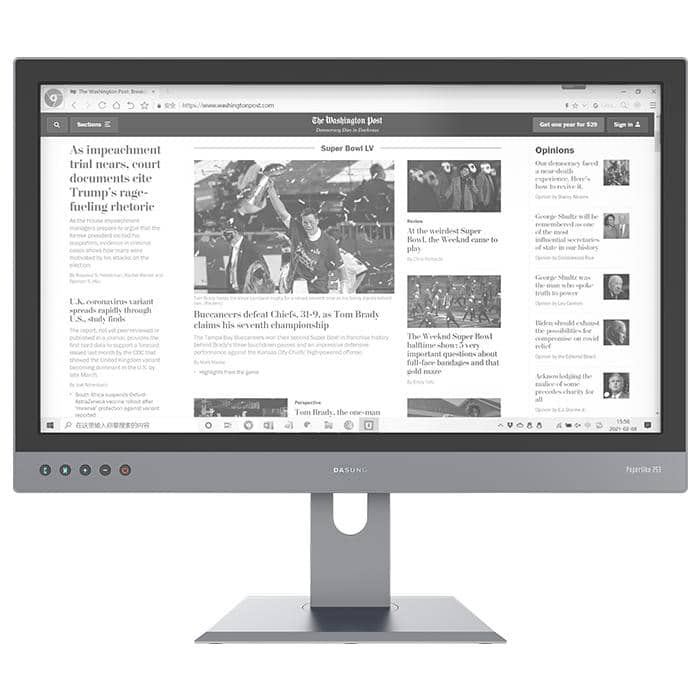
\includegraphics[width=0.4\textwidth]{paperlike.jpg}
\end{figure}

\subsubsection{Peripherals}

One of the core implementations of the Mani Station is the distinct lack of the computer mouse. Inspiration for this decision comes from the philosophy of the text editor Vim.

The Vim ideology encourages avoiding the usage of a mouse when text editing and places an emphasis on efficiency and minimalism. This method encourages a keyboard-centric workflow, allowing users to quickly and precisely explore and change text using only keystrokes. The Vim concept seeks to eliminate hand movement and context switching between the keyboard and mouse by doing away with the necessity for a mouse, thus increasing productivity and encouraging a more concentrated and streamlined user experience \cite{vim}.

This improvement to the text editor is something extended in the design of the Mani Station by removing the use of the mouse. Instead, the desktop is shortcut-based and utilizes tab rotations in order to give the user the ability to interact with all parts of the computer without taking their hands off the home row.

\subsection{Software}
\subsubsection{i3 Window Manager}

i3 is a dynamic tiling window manager designed for X11, a windowing system commonly used on Unix and Unix-like operating systems. Its primary goal is to enable users to manage application windows efficiently, utilizing a tree-like structure to arrange windows within various workspaces. Keyboard-driven controls allow users to quickly and effortlessly navigate through windows and workspaces, making the most of the available screen real estate while minimizing the need for the mouse. This focus on efficient window management, along with its lightweight resource footprint, makes i3 an ideal window manager for hosting the Electron instance in the Mani Station project. Additionally, i3's straightforward and highly configurable nature allows developers to easily tailor the window manager to suit the specific requirements of the Mani Station's desktop environment, ensuring a cohesive and streamlined user experience that aligns with the calm computing principles \cite{i3-guide}.

\subsubsection{Electron}
The primary prototyping platform for the desktop environment was the Electron native application framework. Electron is an open-source framework that enables developers to create cross-platform desktop applications using front-end web code such as HTML, CSS, and JavaScript. It packages the Chromium rendering engine and uses the Node.js runtime to keep the app’s process alive. This integration with the modern Javascript ecosystem allows developers to leverage a vast ecosystem of libraries and packages, while ensuring that the app ships seamlessly to Linux \cite{electron-docs}.

\subsubsection{Vue.js}

In order to build out the application with Electron, we employed Vue.js. With a strong background in Django, we were extremely familiar with the MVC (Model-View-Controller) paradigm of Vue. Vue offered a flexible, modular approach to the desktop, which is exactly what we required, enabling the creation of maintainable and scalable applications. It also hosts a reactive data-binding system and component-based architecture that allows for aesthetic similarity across the entire desktop environment, making it an ideal choice for the Mani Station's desktop environment \cite{vuejs}.

The combination of Vue.js and Electron facilitated rapid prototyping and seamless communication between different components of the desktop environment. Vue.js's comprehensive documentation and active community support proved invaluable during the development process, ensuring that the final product adhered to calm computing principles while maintaining a high level of usability and adaptability.

\subsubsection{RustyHermit}

The ultimate goal for the software implementation of the Mani Station was to write it in Rust and utilize the RustyHermit framework, a lightweight unikernel, as the core of its operating system. RustyHermit offers several key advantages that align with the calm computing principles guiding the project.

As a unikernel, RustyHermit provides a minimalistic, single-address-space operating system, specifically tailored to run a single application, the desktop environment. This approach eliminates the complexity of traditional multi-process operating systems, resulting in reduced overhead and improved performance. Consequently, the Mani Station can focus solely on delivering a calm computing experience without unnecessary distractions or resource consumption, which also allows for more power to be allocated to graphics output and removing a performance bottleneck in the low-spec system \cite{rust-performance}.

Furthermore, RustyHermit leverages the Rust programming language, known for its emphasis on safety, reliability, and efficiency. Rust's unique features, such as its ownership system and strong typing, minimize the likelihood of memory-related bugs and security vulnerabilities. This ensures that the Mani Station offers a stable, secure, and responsive user experience, in line with the project's goals of fostering a more harmonious relationship with technology \cite{rust}.

Unfortunately, due to our lack of Rust knowledge and prowess, and limited time and resources for development, RustyHermit was not implemented in the final prototype. It is a future aspiration for the project and should be the next step when moving away from Electron.

\section{Methodology}
\subsection{Planning}
\subsubsection{Goals}
The axioms behind the design of the Mani Station were laid out initially in prose, allowing room for interpretation, but still requiring that the developer adhere to a set of strict values.
\begin{quote}
A generation is coming to age \\within their poison garden.\\
We do away with all that.\\
Our computer does not run on attention.\\
Our computer waits patiently\\
for your decision and calmly responds.\\
Not only does it not contribute to the deficit;\\
no, it even will (used rightly) grow the supply.\\
This is accomplished simultaneously and \\synergistically
at the levels of software\\ and hardware.
\end{quote}

Success, in terms of the Mani Station, is not solely defined by technical achievements or broad user adoption, although these are certainly significant. Instead, we consider success as the creation of a technological tool that genuinely assists users in their digital activities, without contributing to attention deficit or encouraging unproductive behavior. This entails developing a computer that respectfully waits for user input, responds efficiently, and ultimately enhances the user's cognitive supply, rather than draining it.

In more concrete terms, we may define success as the creation of a standalone personal computer that is able to replace a user’s home machine that is able to complete fundamental computing tasks (see \ref{appendix:tjhsst}), follow the principles of calm computing, while still being performant and practical.

\subsubsection{Project Roadmap}
The development of this project went through many planning phases, the first of which was the vision. A lot of design and research into functional aesthetics went into the design of the project before development even began. We wanted to ensure that the Mani Station had a strong set of principles that laid its foundation which was realized in the first pamphlet (available at \url{https://github.com/afkomputer/ads/blob/main/manistation.pdf})

\begin{figure}[h!]
    \centering
    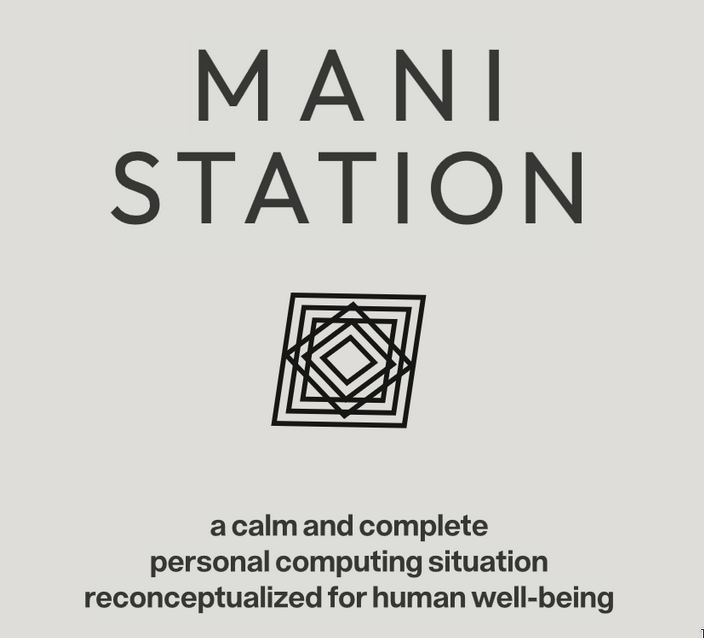
\includegraphics[scale=0.25]{res/pamphlet.png}
    \caption{Cover of advertising pamphlet for the Mani Station}
\end{figure}

This pamphlet also doubled as the first iteration of many design guides for the desktop environment; the reader may notice that the same fonts chosen for the initial pamphlet are the fonts that makeup the sans-serif/serif pairings for the dashboard. Granted, while we may have spent too much time on this pamphlet, it lays out a strong foundation for the proliferation of the original calm design principles in the final product.

This meticulous planning and attention to detail during the initial stages of the project ensured that the Mani Station remained true to its purpose of providing a calm computing experience. By maintaining a steadfast focus on these guiding principles, the project was able to create a harmonious blend of software and hardware components that prioritize tranquility, efficiency, and user-centered design.

\subsection{System Design}

When laying out a roadmap for the project, we needed to get a good understanding of how the system would be built out and designed. Starting from the bottom, considering what kernel, distro, and compositor the Mani Station would host brought about a few criteria. What would be the easiest to spin up for prototyping, what was the most customizable, and most importantly, what was the lightest. The Mani Station ought to be a low-spec device in order to limit noise and disturbance, but it also had to be performant in order to not add any additional lag time to the already slow render rate on the monitor.

\subsubsection{System-level architecture}

These considerations brought about the choice of a custom Debian 11 server instance that was to be stripped of redundant processes in order to maximize screen output. The other consideration was that use of the system should not require the terminal in any situation. This meant that the operating system had to hide all loading and diagnostic information, and transition between screens with the least amount of pixels being printed to the screen \cite{deb11-performance}.

Continuing on, upon first load, the user is walked through a simple onboarding process, and should not have to access the terminal at all. TTY’s are also made harder to access so that the user doesn’t have the opportunity to get lost within the system. Connecting to WiFi and updating services were rendered simply using the nmcli interface.

To further streamline the installation process and enhance the user experience, we employed preseeding techniques with the installation script. Preseeding allows for the customization and automation of the operating system installation by preconfiguring various settings and options, thereby eliminating the need for manual user input during the process. By using a preseed file in conjunction with the installation script, we were able to define the desired system configuration, package selection, and other preferences, ensuring a consistent and optimized setup for each Mani Station deployment \cite{deb11-preseed}. This approach not only facilitated a faster and more efficient installation experience but also contributed to the overall goal of providing a calm computing environment by reducing potential frustrations and time-consuming interactions for the end user.

\subsection{Electron Integration}
By utilizing Electron, the development process of the Mani Station's desktop environment was streamlined and efficient, enabling rapid iteration and testing of various user interface elements and functionalities. This was the case because building a page of the desktop was as simple as writing a website. The framework's support for web technologies facilitated the creation of a highly customizable and responsive user experience, in line with the calm computing principles that guide the project. Additionally, the comprehensive documentation and extensive community resources surrounding Electron further expedited the prototyping phase, ensuring a robust and reliable foundation for the Mani Station's desktop environment. Specifically, to make it best emulate the desktop environment, a few lines of code within the configuration of the window allowed it to seamlessly replace the i3 default.
\begin{verbatim}
    movable: false,
    resizable: false,
    maximizable: false,
    minimizable: false,
    titleBarStyle: 'hidden'
\end{verbatim}

\subsubsection{Dashboard}

When researching different methods for laying out the experience, we returned to the original ideology of minimizing multitasking. This meant that the desktop environment shouldn’t window applications, and it should be difficult to switch between tasks/applications. Since Electron was the platform for the prototype, this meant that we would ideally ship the environment as a single Electron app that would handle context switching and maintain state. Unfortunately, due to performance issues and logistical issues of running sub processes within one Electron instance, the implementation of the final prototype consisted of a separate application for the dashboard and each of the applications.

The dashboard serves as the central hub, hosting essential desktop information, a greeter, an application launcher, a fuzzy search bar for tasks, and the ability to display context from other applications. To ensure a calming and visually appealing user experience, the dashboard was meticulously designed with a streamlined and aesthetically pleasing layout. The initial design was created using Figma design software, enabling rapid iteration and fine-tuning of the interface.

\begin{figure}[!h]
    \centering
    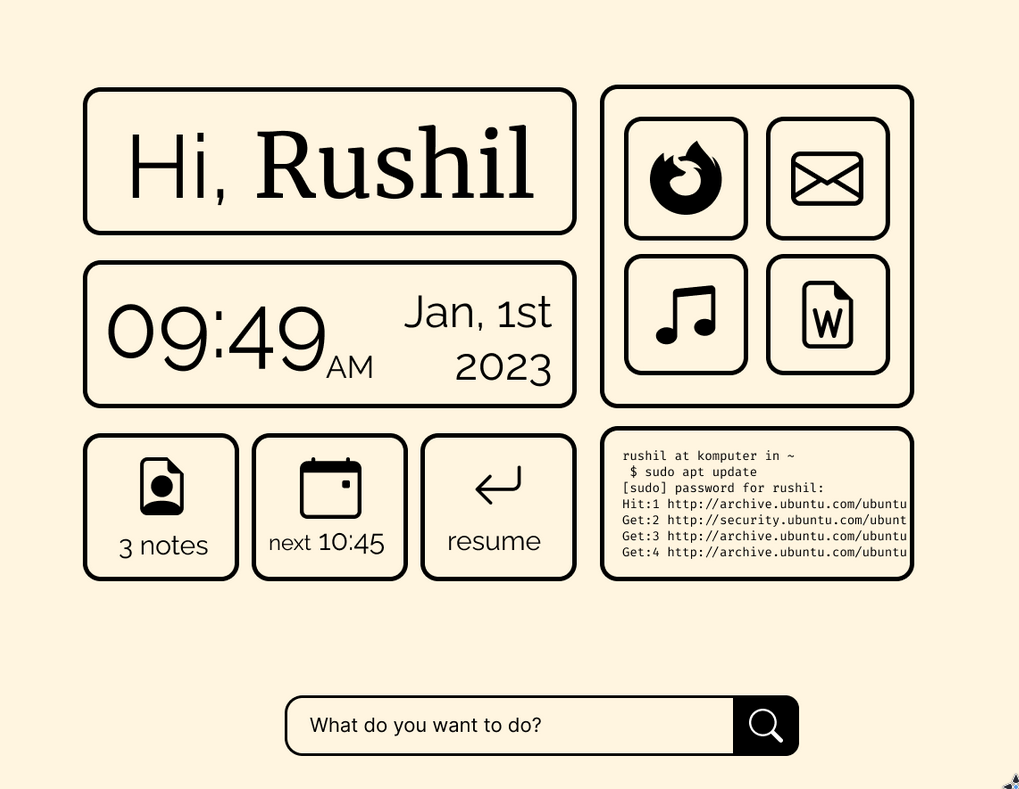
\includegraphics[scale=0.2]{res/dashboard.png}
    \caption{Screenshot of the Mani Station Dashboard}
\end{figure}

The layout features a minimal application launcher in the top right corner, a drop-in terminal in the bottom right, a calendar and to-do list widget in the bottom left, and a centrally located action search bar at the bottom-middle of the screen. The action search bar employs fuzzy search capabilities to assist users in completing tasks on the device, catering to older audiences who may be less familiar with traditional icons.

The primary goal of the search bar is to guide users towards the appropriate application or methodology for accomplishing their entered task. To achieve this, each application is associated with a set of search terms and strings that can be used by the \verb|fzf| algorithm to match the user's input text to the desired application.

\subsection{Core Applications}
Development of the Mani Station’s applications probably took the longest time as each application came with its own implementation challenges. In order to best prioritize what applications would be best for development, we conducted a survey using a randomly sampled group of highschool seniors from Thomas Jefferson High School for Science and Technology (see Appendix A1).
Based on these answers, we can consider the different ways that this sample puts their technology to use, and we come up with the following applications that are necessary for the prototype:

\begin{itemize}
    \item \emph{Web Browser:} A lightweight browser that efficiently renders web pages while adhering to the calm computing principles, focusing on simplified navigation, reduced visual clutter, and resource-conscious operation.
    \item \emph{Document Editor:} A streamlined document editor application that prioritizes ease of use, minimalist design, and essential formatting options to facilitate focused writing and editing without distractions.
    \item \emph{Mail Client:} An intuitive email application that simplifies communication and inbox management, offering a clean interface, straightforward organization, and essential features that align with the principles of calm computing.
\end{itemize}

Finally, a fourth addition, would link the entire operating system together:

\begin{itemize}
    \item \emph{To-Do Manager:} A task management application designed to help users stay organized and on track with their daily tasks and long-term goals. The todo client emphasizes a minimalist interface, intuitive categorization, and easy-to-use input methods, all in line with the calm computing principles, to reduce stress and promote a sense of accomplishment.
\end{itemize}

\subsubsection{Web Browser}
The development of the web browser for the Mani Station posed several challenges and required careful consideration with respect to balancing user safety and user experience. Initially, the idea of developing our own browser was contemplated. However, building a browser from scratch would be an extremely time-consuming task that may have extended to the entire length of the project. It would require handling complex functionality like HTML rendering, JS sandboxing, runtimes, and execution, and CSS interpretation, amongst an array of other tasks.

In this context, \verb|surf| emerged as an interesting alternative. Surf is a simple web client based on GTK+ which has only the ability to display sites and follow links. It was a lightweight, straightforward, and minimalist surfer, focusing primarily on the core functionality of a browser. The XEmbed protocol support made it possible to embed surf into another application which extended its flexibility and possibilities. Moreover, surf’s capability to navigate to different URI by setting its XProperties provided a certain level of control over the browsing experience \cite{surf}. Despite these advantages, surf's simplicity also meant it lacked some of the essential features expected in a modern web browser, such as tabbed browsing, built-in search functionality, and security features. This potential limitation to the user experience led us to explore other alternatives.

Electron's BrowserWindow functionality emerged as a potential solution during our exploration. This module allows for the creation of a new renderer process, which essentially could handle the webpage rendering. It seemed promising as it allowed leveraging web technologies like JavaScript, HTML, and CSS. However, while BrowserWindow handles page rendering, the rest of the browser functionality would still need to be implemented. Basic features such as tabbing, history management, and link following would require custom development. Furthermore, this would create a rather piecemeal browser structure, which could lead to potential stability and compatibility issues down the line. Just like surf, Electron's BrowserWindow started to show similar limitations in terms of comprehensive features and user experience.

Given these considerations, our attention shifted towards pre-existing, feature-rich, and secure open-source browsers. After careful evaluation, we decided on using Qutebrowser. Qutebrowser is a keyboard-focused browser with a minimal GUI, which provides advanced features while maintaining a simple user interface. It also has a robust security model, which is paramount when dealing with web content. Another crucial factor that favored the selection of Qutebrowser was its alignment with our peripheral philosophy, particularly the Vim-like mode of operation that emphasizes keyboard-only use. Qutebrowser incorporates a Vim-inspired interface, supporting a range of keyboard shortcuts for intuitive and efficient navigation. This feature seamlessly complements our focus on keyboard-centric computing, promoting a more focused and efficient interaction paradigm \cite{qutebrowser}.

The integration of Qutebrowser into the Mani Station was a considerable success. It provided users with a full-featured web browsing experience without compromising the calm and focused computing environment we aimed to create. This choice demonstrated that the appropriate selection and adaptation of existing open-source software could meet our specific needs, eliminating the need for impractical development from scratch or potentially insecure solutions.
\subsubsection{Document Editor}
The Document Editor forms a significant part of our application suite, providing tools for both text processing and code editing. In today’s age, both applications are usually a requirement for workflows which is what led us to split the Document Editor into two sub-applications. This decision allows us to tailor each component to its specific use case, optimizing for the unique needs of general text editing and programming respectively.
\paragraph{Word Processor}
In developing the word processor for the Mani Station, we sought a solution that would offer comprehensive functionality while adhering to the principles of calm computing. We found that answer in LibreOffice Writer, an open-source word processor that has earned a strong reputation for its powerful features and compatibility with various document formats \cite{writing-in-linux}.

Given that LibreOffice Writer is open source, we were able to create a fork of the project in order to tweak the feature and look to our specifications. A key aspect of calm computing is reducing screen clutter and visual distractions. To this end, we streamlined the interface of LibreOffice Writer, simplifying toolbars and removing non-essential elements.This came about through a combination of theming and preference editing to reduce animations and forcing pagination rather than scrolling. We wanted to edit application code as well, but LibreOffice Writer has its UI laid out in C++ which was a language that I was less familiar with for this application.
\paragraph{Code Editor}
The code editor is another crucial component of the Mani Station, providing a tool for users to write and debug code efficiently. For this task, we chose Sublime Text 4, a highly customizable and versatile text editor that is widely praised for its speed, ease of use, and powerful features. Much like our approach with LibreOffice Writer, we took advantage of Sublime Text's plasticity to align it with the principles of calm computing \cite{sublime}. 

In our initial customization efforts, we implemented a minimalist theme with subdued colors and simplified icons to reduce visual clutter. We further streamlined the interface by removing seldom-used elements such as certain toolbars and panels. In parallel, we addressed animations and transitions, disabling or toning down features like smooth scrolling and highlight animations, considered superfluous for our calm computing environment. This resulted in a tranquil, focused workspace conducive to productivity.

Users can write, debug, and understand code with greater focus, benefiting from the full suite of Sublime Text's features without unnecessary distractions.
\subsubsection{Mail Client}
For the Mani Station's mail client, we elected to utilize the Geary mail client, an application developed in GTK for the GNOME operating system. Our selection of Geary was grounded in its inherent simplicity and the customization opportunities it affords, allowing us to align the application with our calm computing principles \cite{geary}.

Geary's straightforward interface and user-friendly functionality made it a suitable starting point for our project. We leveraged its customizability to strip back extraneous elements, reducing visual clutter and promoting a serene, focused user experience. This involved re-skinning the client, removing rarely used toolbars and panels, and muting colors to create a tranquil, distraction-free workspace.

Despite the success of the Geary-based mail client, we are always open to exploring new possibilities for enhancement. One such avenue for future development is the implementation of "mutt," a small but very powerful text-based mail client. Its use could provide an even more streamlined and keyboard-centric user experience, aligning with our overarching goal of creating a calm computing environment on the Mani Station.
\subsubsection{To-Do Manager}
The development of the to-do app for the Mani Station was initiated by following an online tutorial titled "Build a Todo App with Electron." This provided the basic framework for the application. To enhance functionality, we integrated the app with the Todoist API, enabling synchronization with cloud-based tasks \cite{todo-electron}\cite{todoist}.

A key aspect of this development was the use of Datastore.js, a JavaScript database library. This allowed the to-do app to interact seamlessly with other applications on the Mani Station, such as the dashboard, which could display to-do information contextually, enhancing the user's overview of their tasks.

This approach of inter-application communication was fundamental in our goal to create a harmonious, integrated software ecosystem. By enabling applications to access and present shared data, we could build a more user-friendly, cohesive experience, with the to-do app serving as an example of this philosophy. The integration fostered by Datastore.js is a significant step towards developing applications that are specifically tailored for the Mani Station, promoting a calm computing environment.
\section{Results}
\subsection{Introduction}
The results section aims to evaluate the success of the Mani Station based on the goals outlined in 4.1.1. It should be noted that the current iteration of the device as of publication is a prototype intended for proof-of-concept.
\subsection{User Experience Feedback}
The design approach and careful consideration of our values shaped the Mani Station’s user experience. From the omission of the mouse, to the lack of a typical large computer tower, to the lack of backlight and low refresh rate, users took notice to a slew of changes that the Mani Station presented.

Users were asked to respond to an email from a professor asking for further research on a topic of their choice by finding information online, typing up a paragraph response, and formulating an email response using the Mani Station. They were then tasked with doing the same on their personal device of choice.

Surprisingly, during first trials, users reported an average increase in stress when asked to complete these tasks within a time limit. When asked for further comments, users reported a high initial learning curve and difficulty of use as the layout was slightly foreign. This was expected as standard personal computer users would have trouble understanding other types of computing systems and feel comfort when doing the same task on their own machines.

Each of the subjects were asked to do same set of tasks again between 1-3 days later, and while some users still found the machine slightly difficult to use due to lack of familiarity, across the board we noticed that users actually felt more calm and less distracted when completing tasks on the second go around. One user, whose control device was their mobile phone, actually paused during the second experiment to respond to a text that they had received.

Feedback on the customizations and simplifications of the applications were also well received. The minimalist themes in the Document Editor and the Web Browser we noted for reducing visual clutter and distractions.

In conclusion, despite an initial learning curve and stress increase observed in first-time users, the Mani Station's unique approach to user experience marked by a departure from conventional computing methods led to more focused and calm user interactions in subsequent uses.
\subsection{Performance}
In terms of raw hardware performance, the Mani Station is not intended to compete directly with traditional Windows machines or other personal computers. The low refresh rate e-ink display and minimalistic hardware setup deliberately step away from the typical power-centric approach. While this might have resulted in slower load times or less dynamic animations when compared to a Windows PC, it's important to note that these are intentional design decisions aimed at reducing distractions and fostering a calmer computing environment.

Nevertheless when base loads were compared between a Dell Latitude 3300, This machine was one of many provided by Fairfax County Public Schools to all current highschool students, running Windows 10 Education, we noticed a 249.2\% decrease in CPU usage and a 132\% decrease in RAM usage. This was mainly due to the fact that Windows OS includes a myriad of background services, telemetry, and startup applications unbeknownst to the user. Our operating system sustains a majority of its load from the Xorg compositor as observed using the htop utility.

The refresh rate of the monitor is not provided by the manufacturer, and we did not have proper tools or methodology for testing a base refresh rate. Along with this, the monitor does not refresh the entire screen in the standard fashion as one might expect, instead portions of the screen are refreshed when it is changed. Therefore, we do not have a firm quantitative analysis for the comparison of our monitor compared to a typical 60Hz computer monitor.
\subsection{Implementation Analysis}
In developing the Mani Station, we chose to adapt established applications—web browser, document editor, mail client, and to-do app—to suit our calm computing environment. This approach enabled us to utilize their proven functionality while customizing their user interfaces to match our design ethos. Additionally, the integration of these applications via Datastore.js showcases the potential for a cohesive software ecosystem, vital for Mani Station's future development.
\subsection{Conclusion}
The Mani Station's trial results indicate its potential as an effective tool for calm computing. While initial usage yielded reports of a steep learning curve and heightened stress, repeated exposure demonstrated a significant shift towards a calmer and less distracted user experience. It's noteworthy that the station's design elements, such as the keyboard-only navigation, minimalistic themes, and lack of visual clutter, were positively received. This highlights the user's adaptability and the potential benefits of breaking away from traditional PC paradigms in favor of an environment conducive to productivity and tranquility.
\section{Final Remarks}
As we reflect on the journey of creating the Mani Station, we are deeply grateful for the opportunity to have been a part of this unique project. It has truly been a labor of love, brought to life by the integration of diverse skills, viewpoints, and relentless dedication from everyone who helped along the way. We were not just developers or engineers; but designers, psychologists, and philosophers, wearing each hat interchangeably as we manifested the vision of calm computing.

The multiple dimensions of knowledge and skill required for this project provided a holistic perspective, considering not only the technological facets but also the sociological, psychological, and aesthetic aspects of the design decisions. This unique intersectional approach greatly influenced the Mani Station's design, grounding it in principles that prioritize user experience and wellbeing.

As I envision the future trajectory of the Mani Station, a few key objectives stand out. A prominent goal is to build and develop our core applications from scratch. While we have currently adapted and customized existing applications, creating applications that are natively designed for calm computing will enhance the authenticity and efficacy of the Mani Station experience.

The endeavor to develop our own E-ink monitor represents a significant technological challenge but is vital to maintain the integrity of our design philosophy. An E-ink monitor designed specifically for the Mani Station will be optimized to work with our unique hardware-software ecosystem, improving the overall user experience.

Beyond just the technological developments, I believe that the Mani Station holds immense potential for customization and adaptation to specific applications. For instance, deploying customized Mani Stations in libraries could potentially revolutionize the library experience, aligning the calm computing principles with the inherent tranquility and focus required in such environments.

Similarly, designing a version of the Mani Station specifically for elderly homes could drastically improve their interaction with technology, offering a calm, straightforward, and less distracting computing experience.

In essence, the future of the Mani Station presents a multifaceted approach that merges technological advancements, user-centric designs, and adaptive deployments. This endeavor to continue pushing the boundaries of calm computing holds immense promise for shaping the landscape of human-computer interaction.

\section*{Appendix}
\appendix
\section{TJHSST Technology Use Survey Results}\label{appendix:tjhsst}
Every student was asked, “If you could only have one application on your computer, what would it be?” Here are the results of that survey:
\begin{figure}[h!]
    \centering
    \caption{Survey for Single Application}
\rowcolors{2}{gray!25}{white}
    \begin{tabular}{lc}
    \rowcolor{gray!50}
    Total(n)                        & 42 \\
    Web Browser                     & 17          \\
    File / Task Manager / Utilities & 9           \\
    Video Games / Other             & 11          \\
    Word Processor / Code Editor    & 5  
\end{tabular}
\end{figure}


In the initial survey, the responses from the high school seniors at Thomas Jefferson High School for Science and Technology were diverse. While a significant portion of the responses included various video games, these cannot be discounted as they reflect a genuine interest among this age group. Further analysis revealed three main categories of responses: web browsers, operating system utilities, and code editors. Interestingly, "Task Manager" was mentioned by three distinct individuals, demonstrating the importance of system monitoring tools even among younger users.

Given the versatile nature of web browsers, a follow-up survey was conducted with a different group of seniors from the same school. The results were as follows:
\begin{figure}[h!]
    \centering
    \caption{Survey for Single Website}
\rowcolors{2}{gray!25}{white}
    \begin{tabular}{lc}
    \rowcolor{gray!50}
    Total(n)                        & 14 \\
    YouTube / Social Media / Web Games                     & 6          \\
    Email & 3           \\
    Learning Management System & 1          \\
    Search Engine    & 4  
\end{tabular}
\end{figure}

The responses indicate a significant interest in social media sites and web games, once again highlighting their importance to this age group. However, focusing on more productivity-oriented applications, we can categorize these responses into three main groups: email, learning management or work platform, and search engines.

These findings suggest that while recreational use of technology is prevalent among younger users, there is also a strong need for more task-oriented applications. Further research would be necessary to fully understand these preferences and to avoid any potential bias in the interpretation of the data.

{\footnotesize \bibliographystyle{ieeetr}
\bibliography{proposal}}

\end{document}







